\chapter{Experimental evaluation}\label{chapter:experimental_evaluation}

In this chapter we propose a set of experiments to study the performance and scalability of both our distributed framework for CER and our distributed evaluation algorithm. This study aims to show that the claims of our work empirically hold. This chapter is organized as follows. First, we describe our implementation. Then, we describe the design and set up of our experiments, including how we generated the synthetic data and the characteristics of the system. Then, for each experiment, we describe the experiment and discuss the results. Finally, we summarise the main conclusions of the chapter.

\section{DCORE in a nutshell}\label{chapter:dcore}

In this section, we review some implementation details of DCORE. We implemented DCORE to run on the JVM \cite{jvm}. Its code is open-source and available at \url{https://github.com/dtim-upc/DCORE} under the GNU GPLv3 license. DCORE implementation depends on a fork of \href{https://github.com/dtim-upc/CORE2/tree/distributed_enumeration}{CORE}. This fork implements our novel distributed evaluation algorithm.

\textbf{CORE.} CORE is implemented in Java 11 and has some clever optimizations. For example, complex predicates are encoded in an efficient array representation and are only evaluated once during the execution of the algorithm. Another example is I/O-determinization which is run \emph{on the fly} are many of the steps are cached and only computed once. Another example is memory management. Nodes in the tECS data structure are weakly referenced, while the strong references are stored in a list that is pruned once in a while taking into account nodes that are outside the time window, allowing the garbage collector to reclaim that memory without the need to modify the tECS data structure.

\textbf{DCORE.} DCORE is implemented in Scala 2.12 \cite{scala}. Scala \cite{scala} is a statically typed programming language that fuses object-oriented and functional programming, which can freely interoperate with Java. DCORE is built on top of Akka \cite{akka} (Akka Cluster in particular). Akka is a set of open-source libraries for designing scalable, resilient system that span processor cores and networks. Akka’s use of the actor model provides a level of abstraction that makes it easier to write correct concurrent, parallel and distributed systems. DCORE depend on several libraries that are downloaded and compiled using Sbt \cite{sbt}. Sbt is a typesafe and parallel build tool for Scala and Java projects. Sbt guarantees reproducibility of the compilation of the project. As mentioned before, DCORE depends on our own fork of CORE that implements the novel distributed evaluation algorithm. DCORE is built as a Command-line interface program and has many available parameters. The landing page of the project has a detailed explanation on how to compile and run the project. We remark that we made an effort to guarantee that the implementation is correct and outputs the expected result. We designed several automated tests to validate that the implementation is close to the specification.

\section{Experimental setting}\label{sec:setup}

% Comment that we run the experiments on a single physical machine because there should be noticeable differences.
% But we should validate this hypothesis in future work.

% Explain how the queries and the workload is generated.

% Explain the three queries (like in CORE).
% Q1: A;B;C
% Q2: A;B+;C
% Q3: A+;B+;C

\textbf{Reproducibility}. Explain that this is open-source, https://reproducibility.sigmod.org/

\section{Experiments on the evaluation of complex predicates}\label{sec:predicates}

% Subfigure and place them together ?

% A;B;C
\begin{figure}[H]
  \centering
  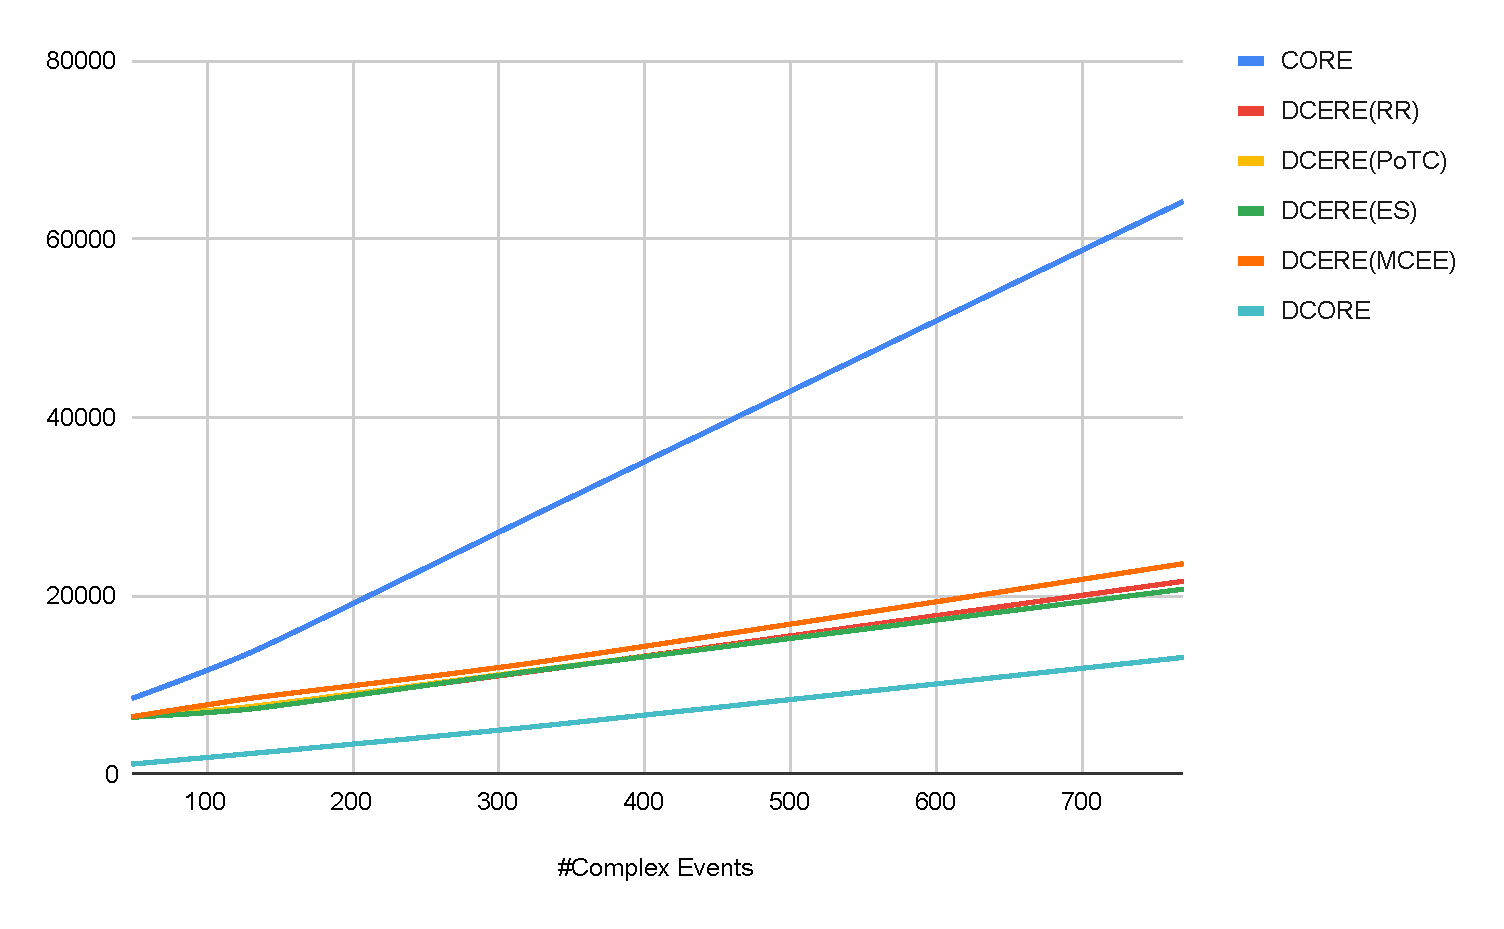
\includegraphics[scale=0.5]{experiment_1_chart_3}
  \caption{$Q_{1}$.}
  \label{fig:???}
\end{figure}

% A;B+;C
\begin{figure}[H]
  \centering
  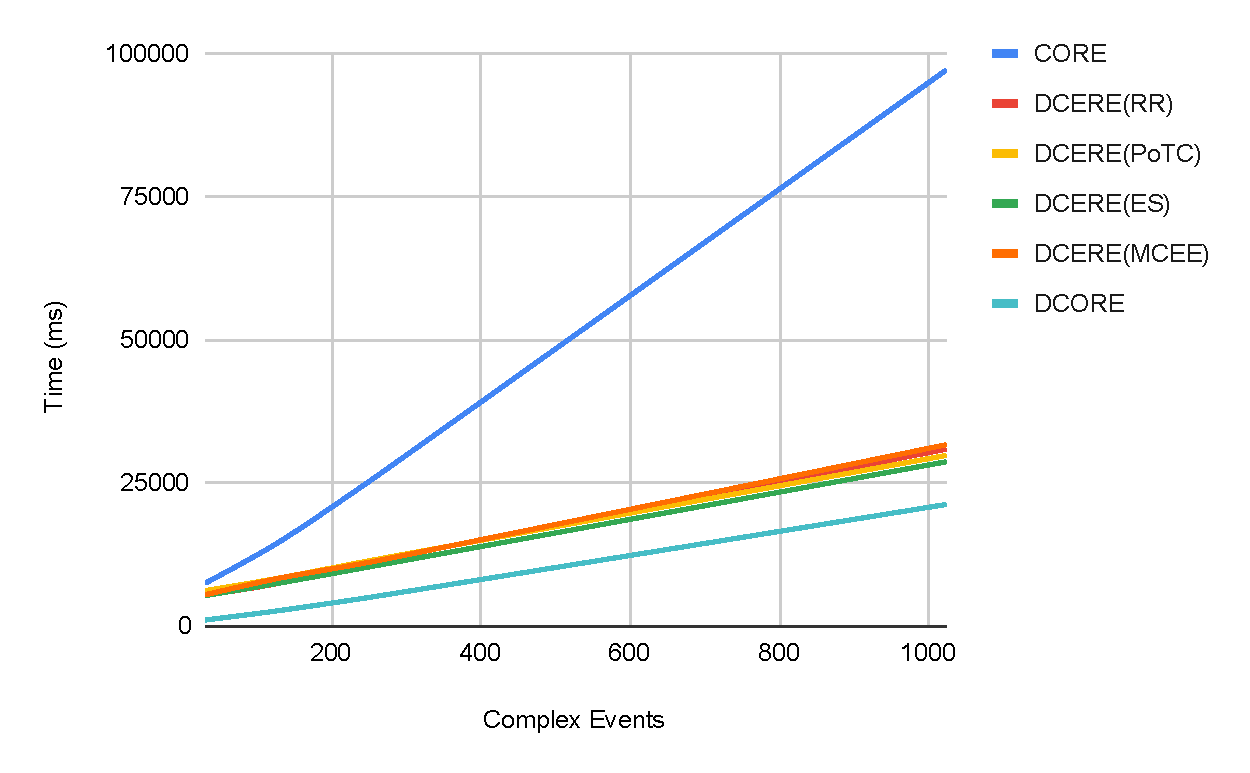
\includegraphics[scale=0.5]{experiment_1_chart_2}
  \caption{$Q_{2}$.}
  \label{fig:???}
\end{figure}

% A+;B+;C
\begin{figure}[H]
  \centering
  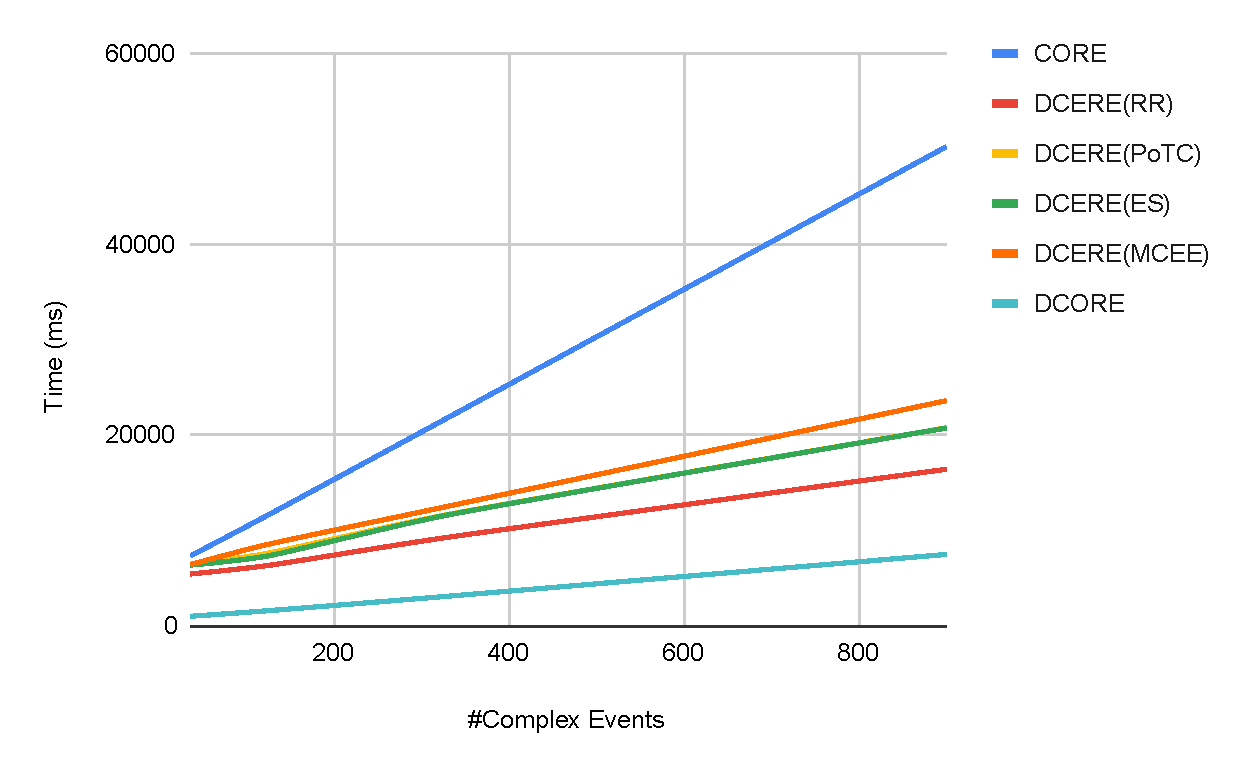
\includegraphics[scale=0.5]{experiment_1_chart_1}
  \caption{$Q_{3}$.}
  \label{fig:???}
\end{figure}


\textbf{Experimental results}.

\section{Experiments on the scalability of the framework}\label{sec:scalability}

% A;B;C
\begin{figure}[H]
  \centering
  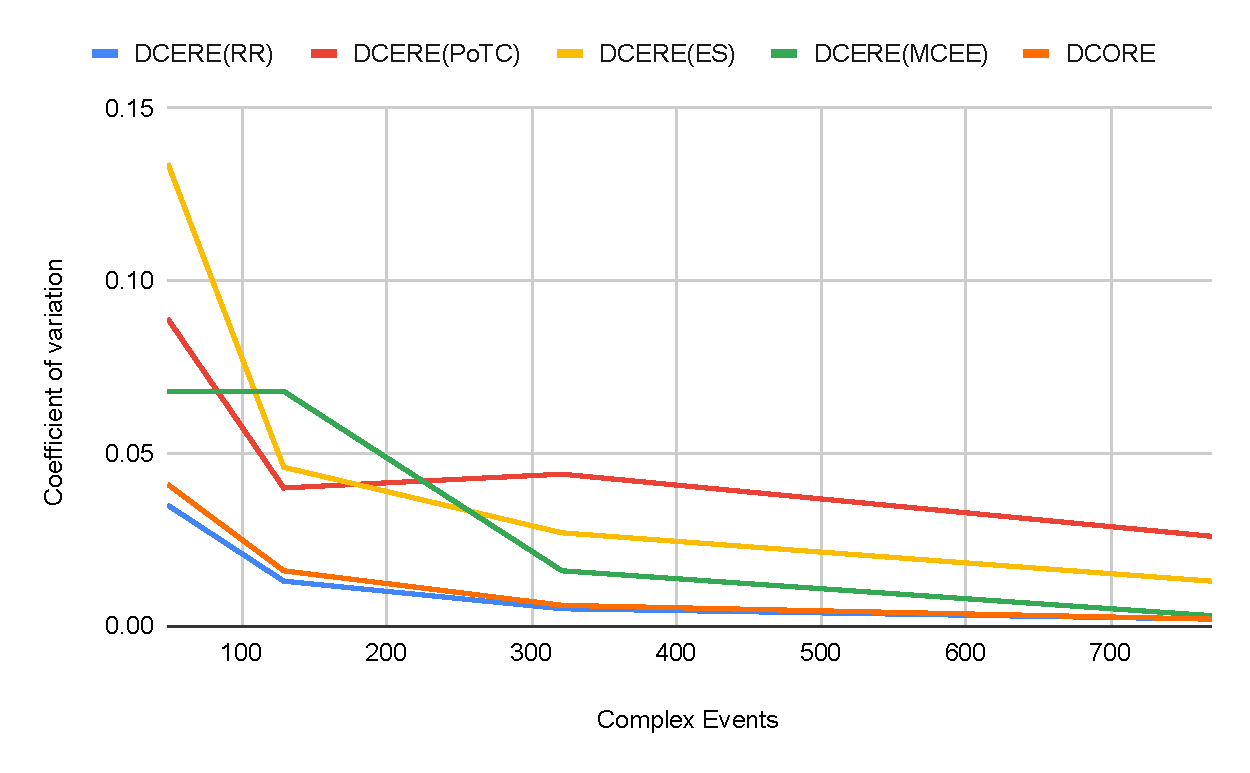
\includegraphics[scale=0.5]{experiment_2_chart_3}
  \caption{$Q_{1}$.}
  \label{fig:???}
\end{figure}

% A;B+;C
\begin{figure}[H]
  \centering
  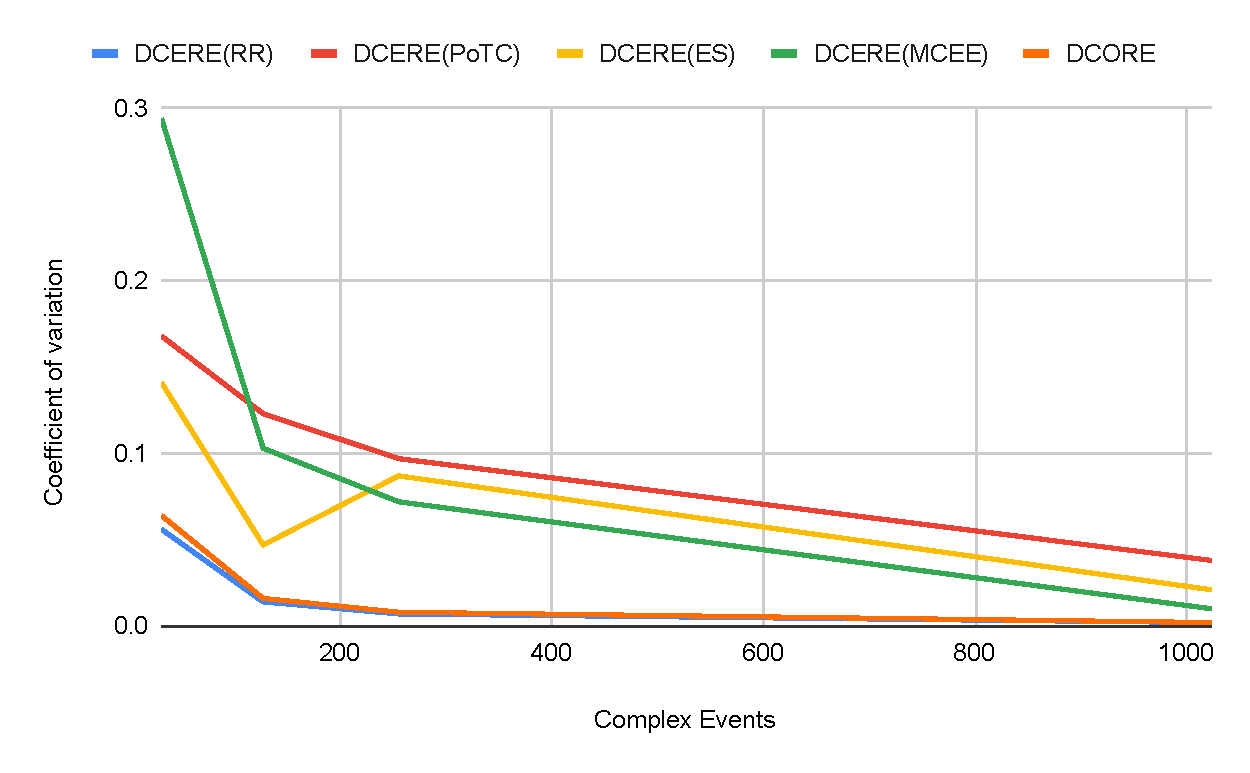
\includegraphics[scale=0.5]{experiment_2_chart_2}
  \caption{$Q_{2}$.}
  \label{fig:???}
\end{figure}

% A+;B+;C
\begin{figure}[H]
  \centering
  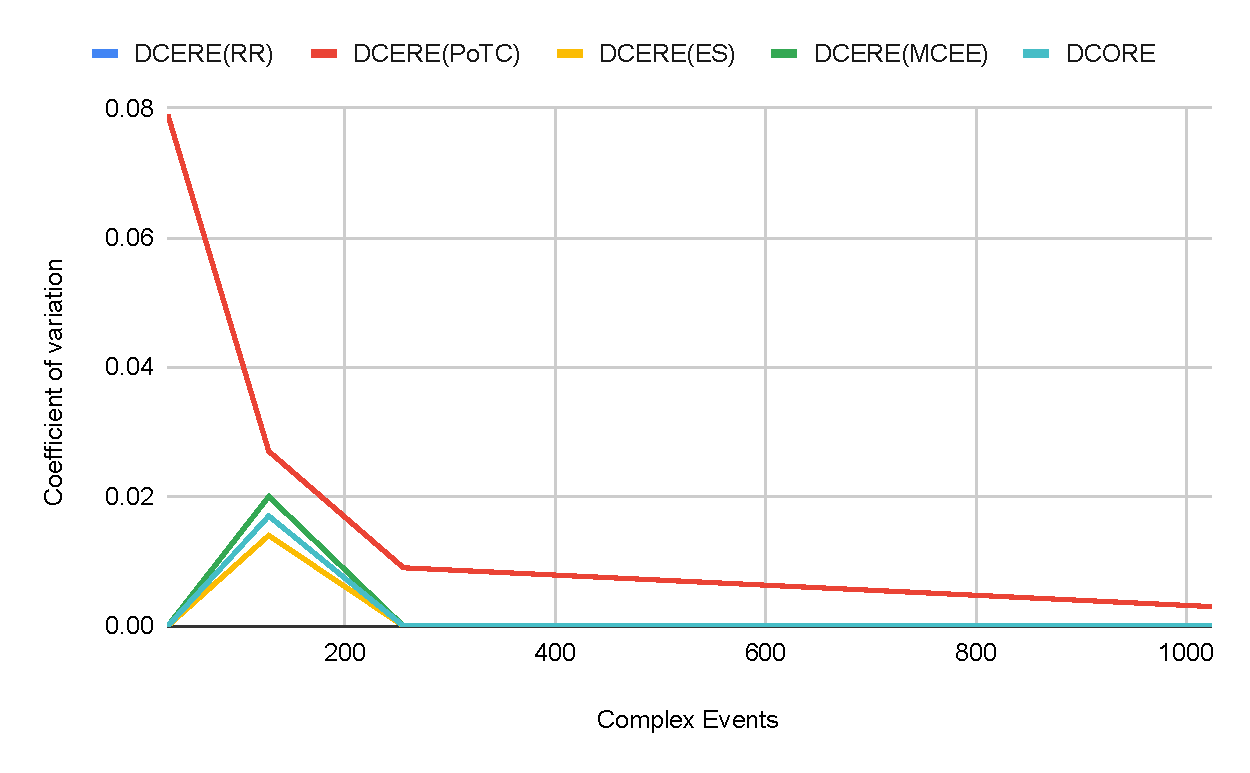
\includegraphics[scale=0.5]{experiment_2_chart_1}
  \caption{$Q_{3}$.}
  \label{fig:???}
\end{figure}



\begin{figure}[H]
  \centering
  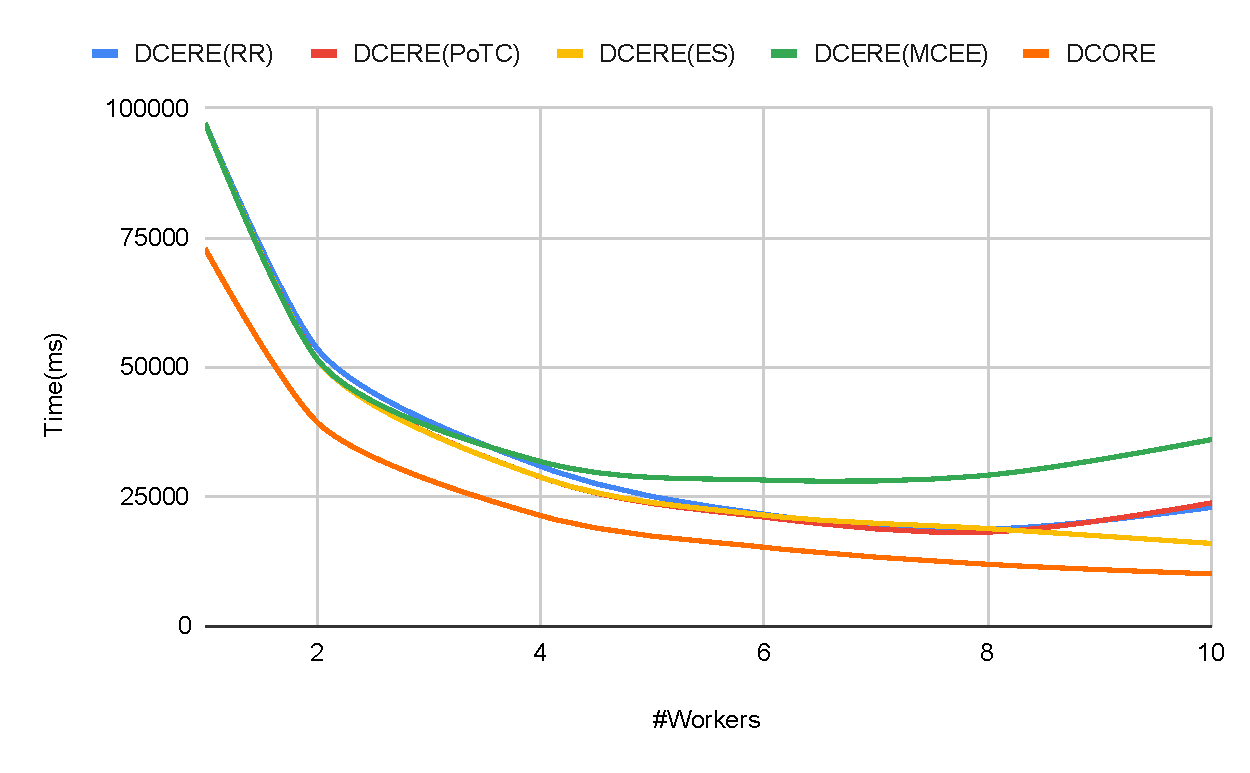
\includegraphics[scale=0.5]{experiment_3_chart_1}
  \caption{$Q_{2}$.}
  \label{fig:???}
\end{figure}

\begin{figure}[H]
  \centering
  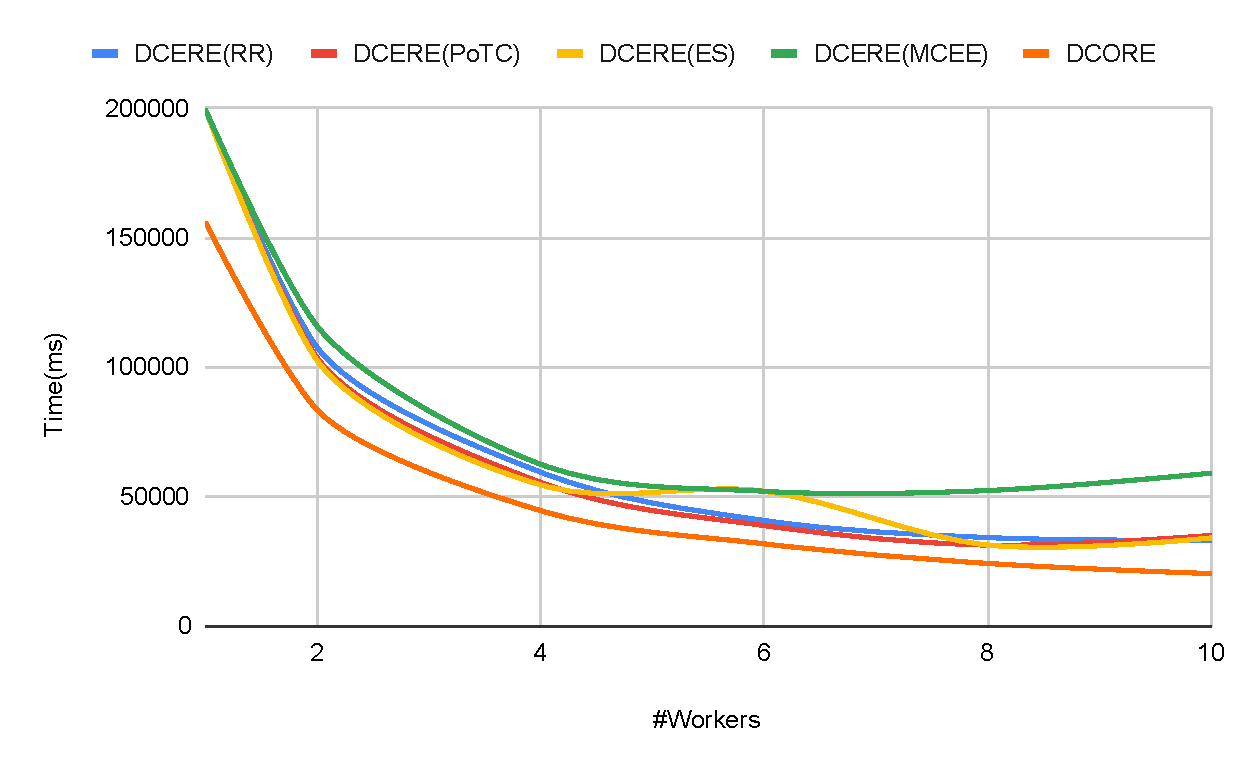
\includegraphics[scale=0.5]{experiment_3_chart_2}
  \caption{$Q_{2}$.}
  \label{fig:???}
\end{figure}

\textbf{Experimental results}.

\section{Experiments on the novel evaluation algorithm}\label{sec:new-algorithm}

% A;B;C
\begin{figure}[H]
  \centering
  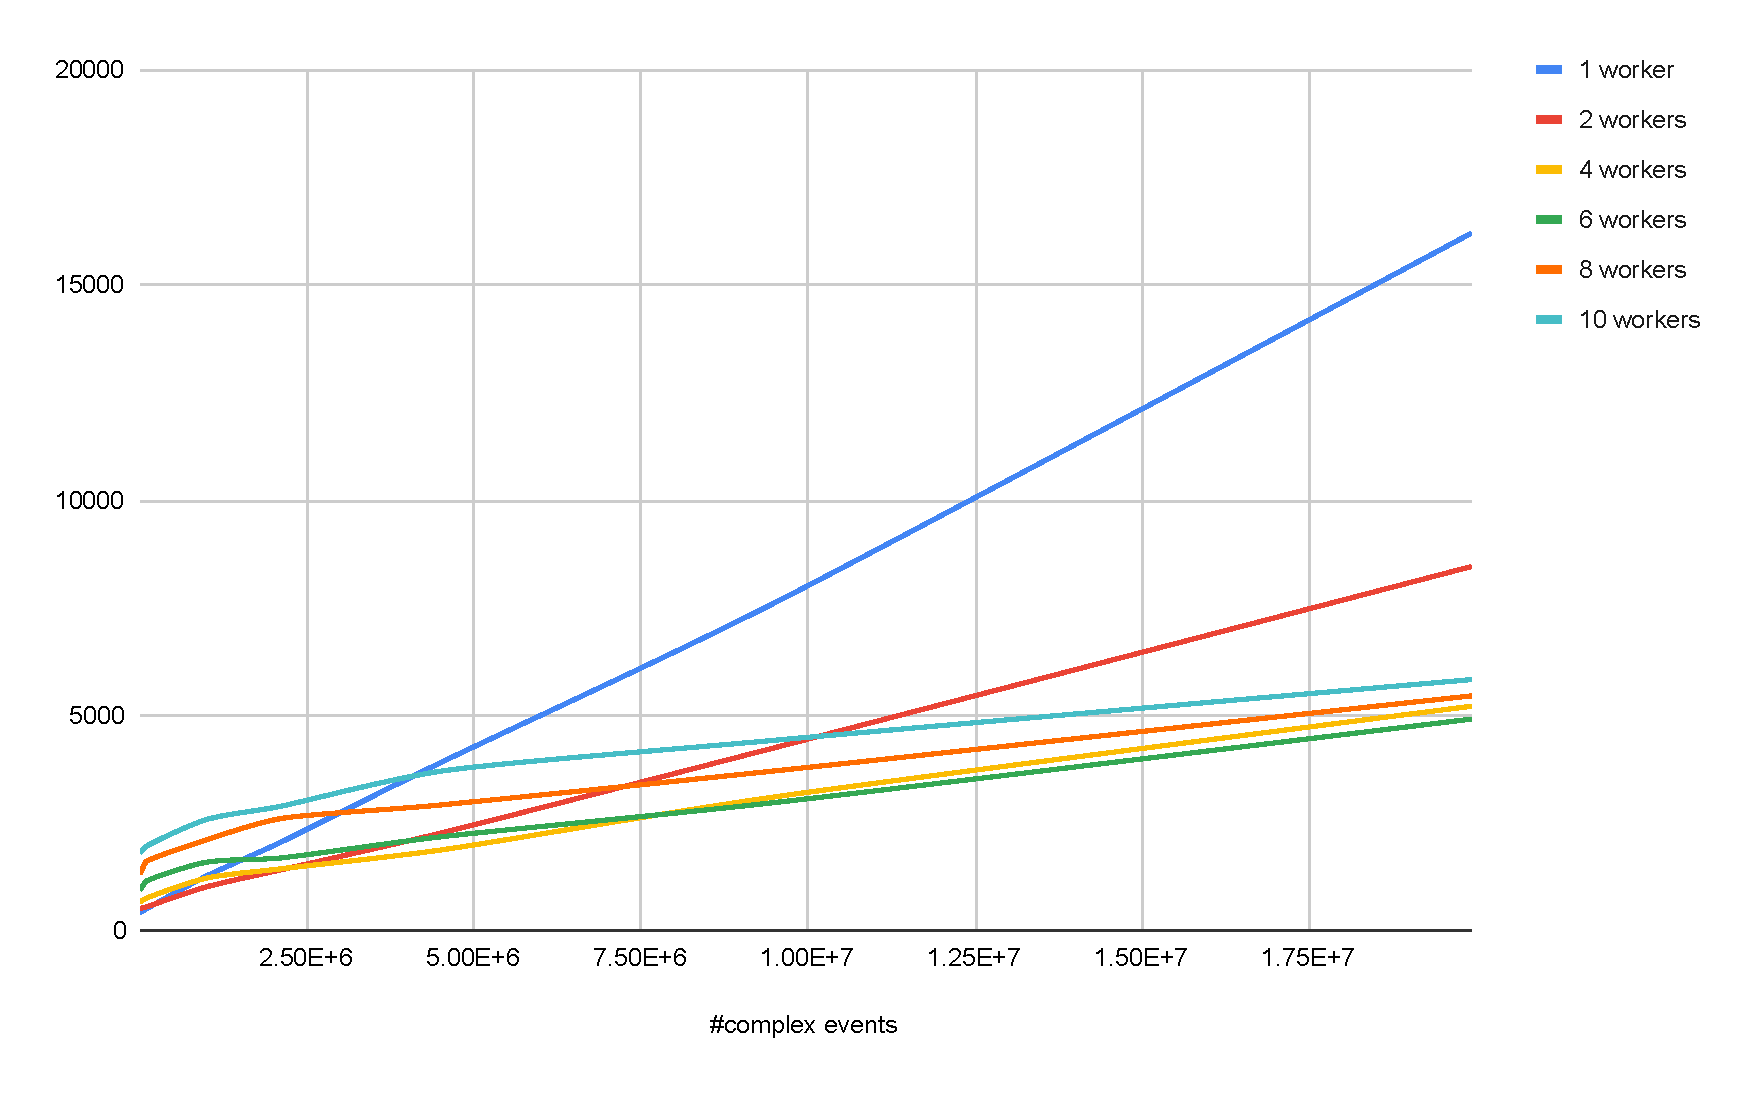
\includegraphics[scale=0.5]{experiment_4_chart_3}
  \caption{$Q_{1}$.}
  \label{fig:???}
\end{figure}
% A;B+;C
\begin{figure}[H]
  \centering
  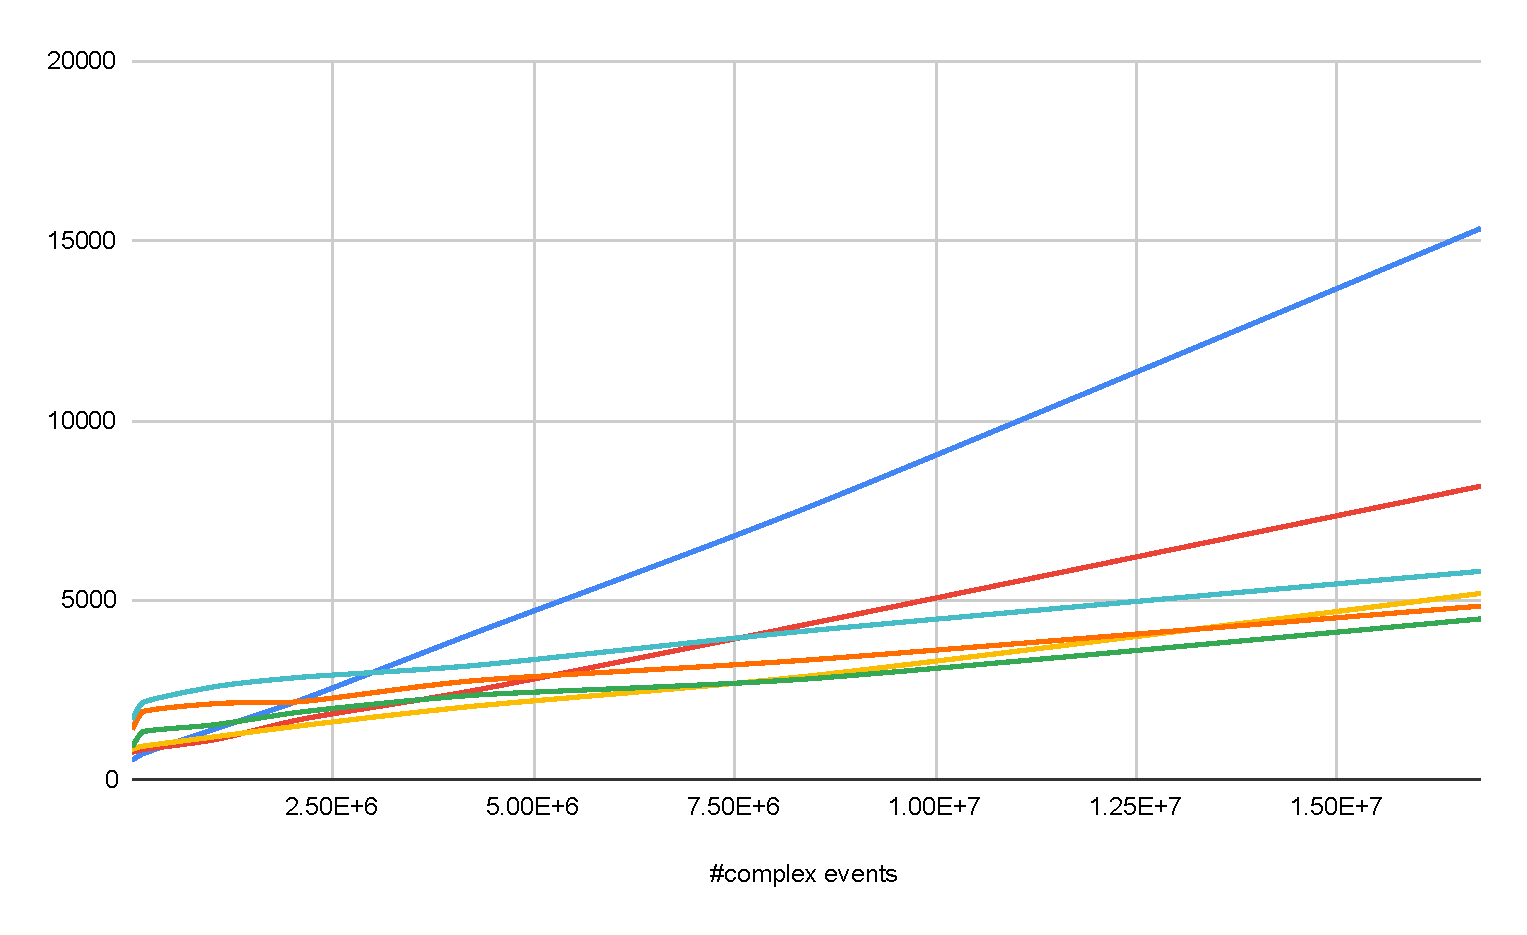
\includegraphics[scale=0.5]{experiment_4_chart_2}
  \caption{$Q_{2}$.}
  \label{fig:???}
\end{figure}
% A+;B+;C
\begin{figure}[H]
  \centering
  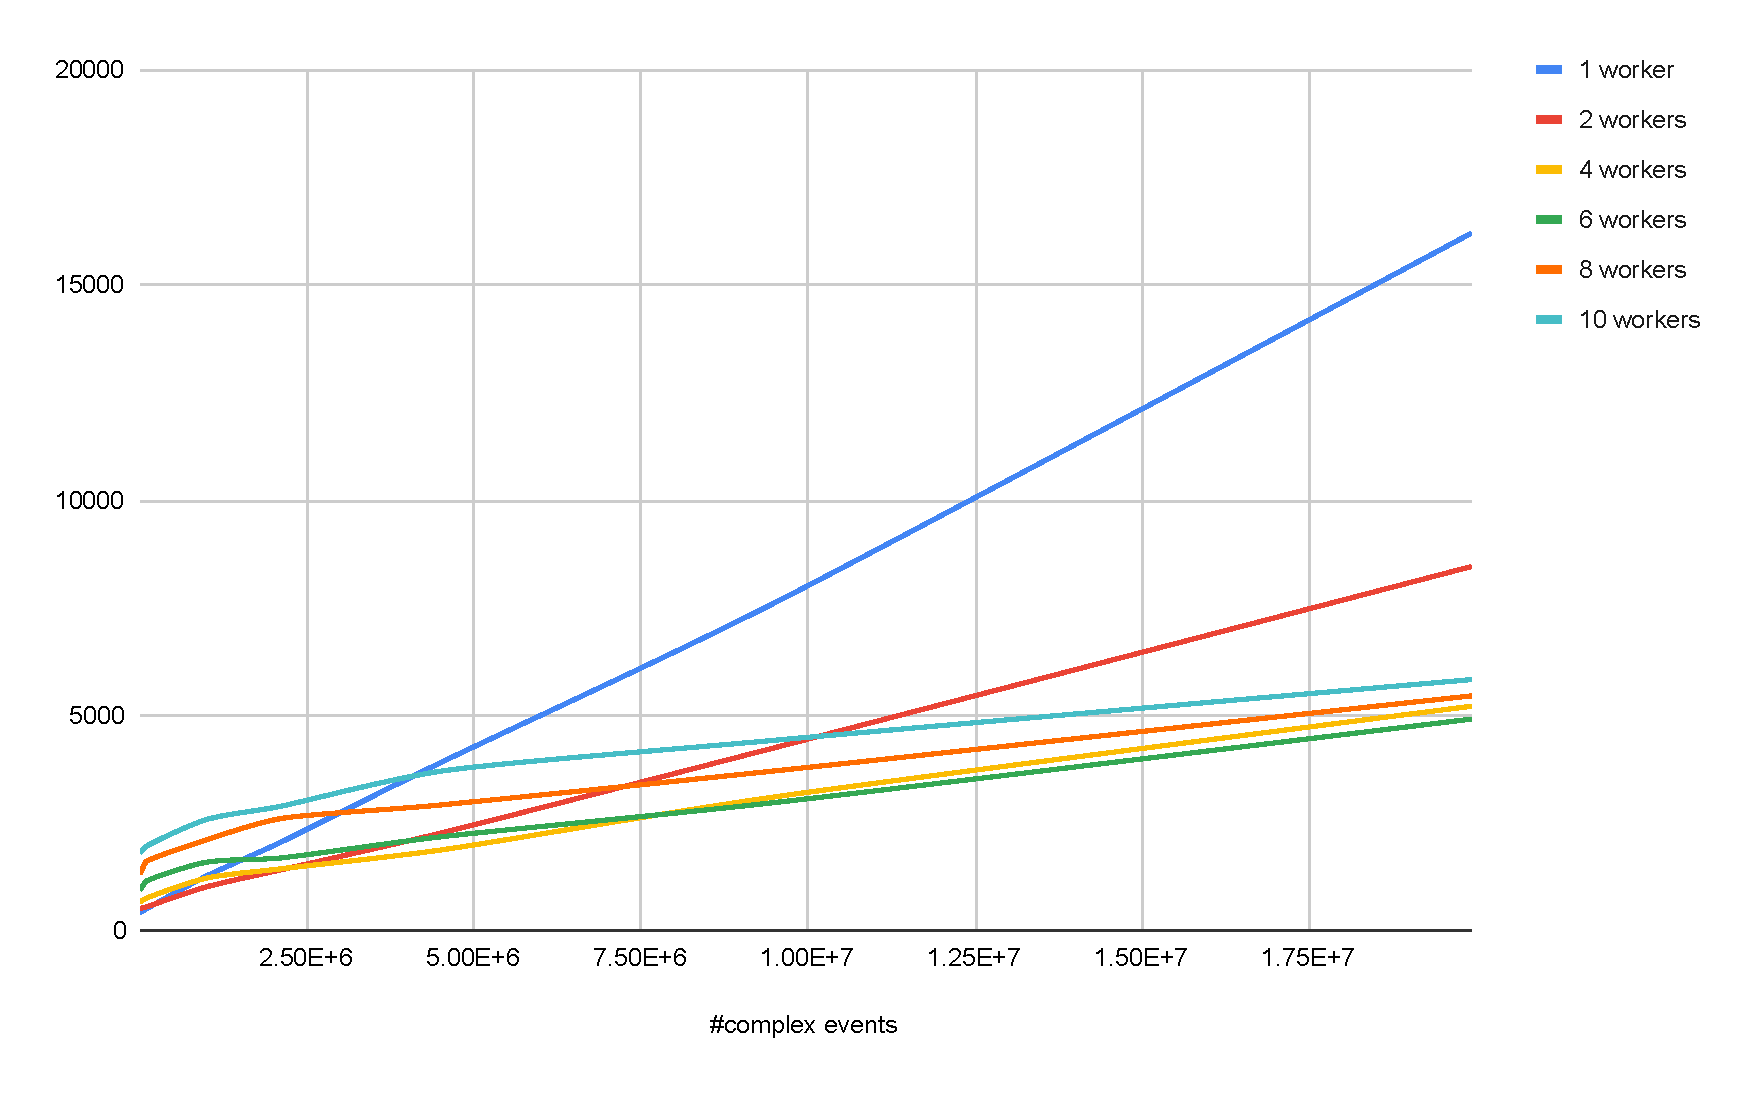
\includegraphics[scale=0.5]{experiment_4_chart_3}
  \caption{$Q_{3}$.}
  \label{fig:???}
\end{figure}


\begin{figure}[H]
  \centering
  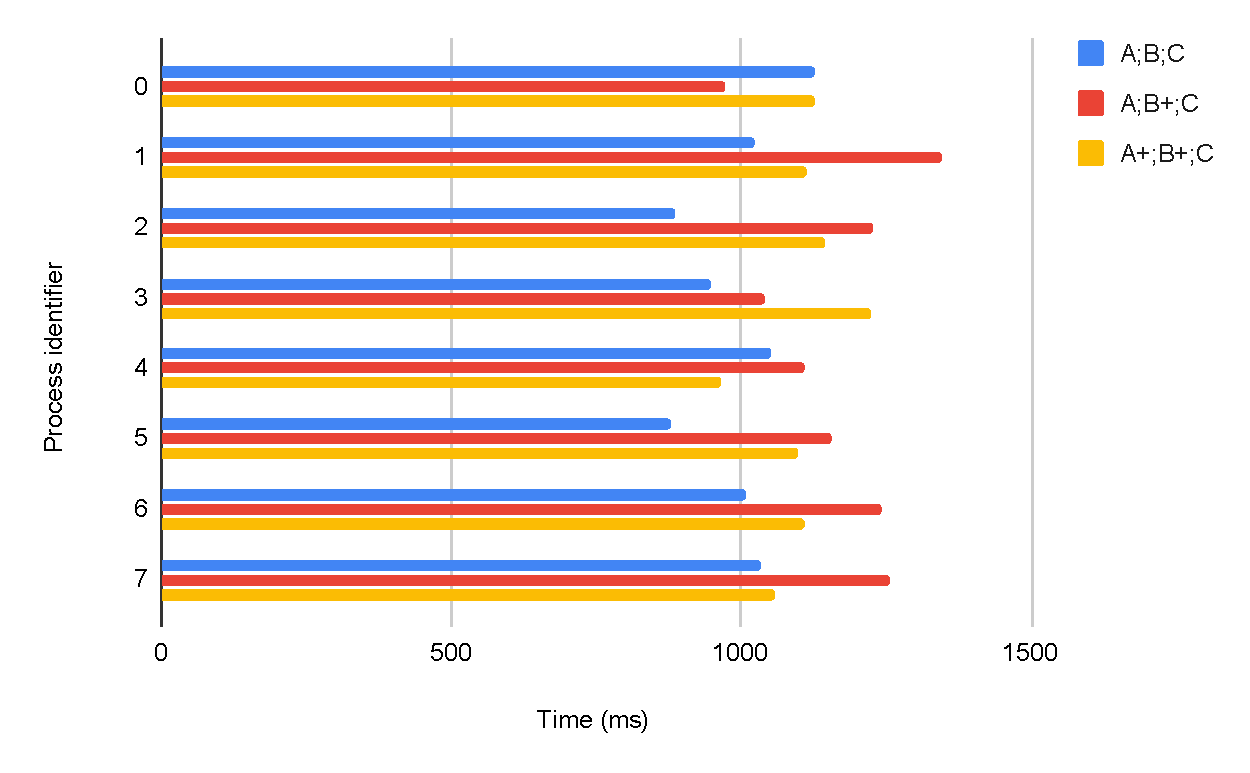
\includegraphics[scale=0.5]{experiment_5_chart_1}
  \caption{.}
  \label{fig:???}
\end{figure}

% 2 processors
\begin{figure}[H]
  \centering
  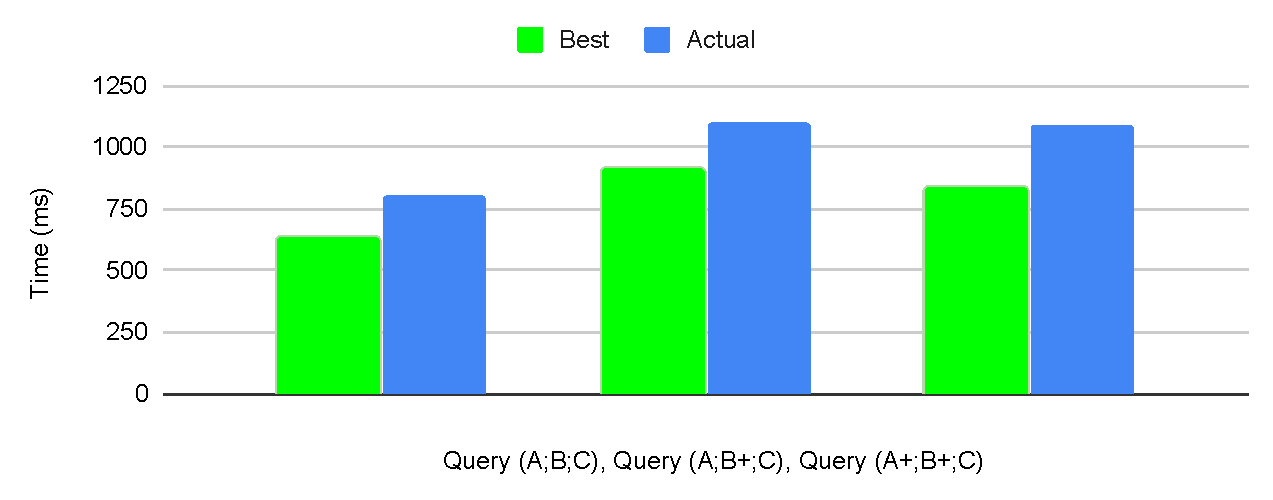
\includegraphics[scale=0.5]{experiment_5_chart_2}
  \caption{.}
  \label{fig:???}
\end{figure}

% 4 processors
\begin{figure}[H]
  \centering
  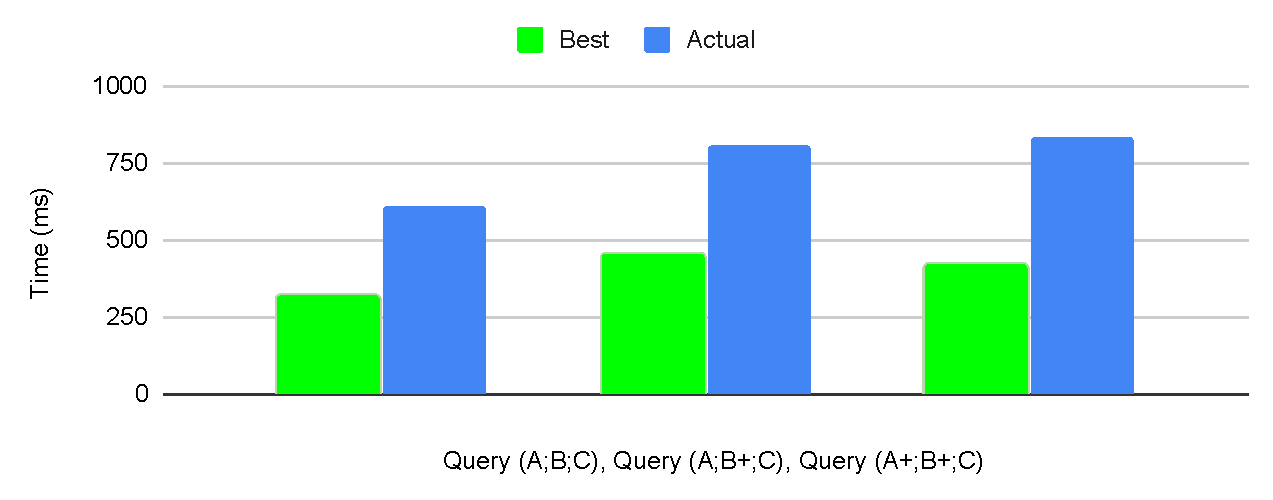
\includegraphics[scale=0.5]{experiment_5_chart_3}
  \caption{.}
  \label{fig:???}
\end{figure}

% 6 processors
\begin{figure}[H]
  \centering
  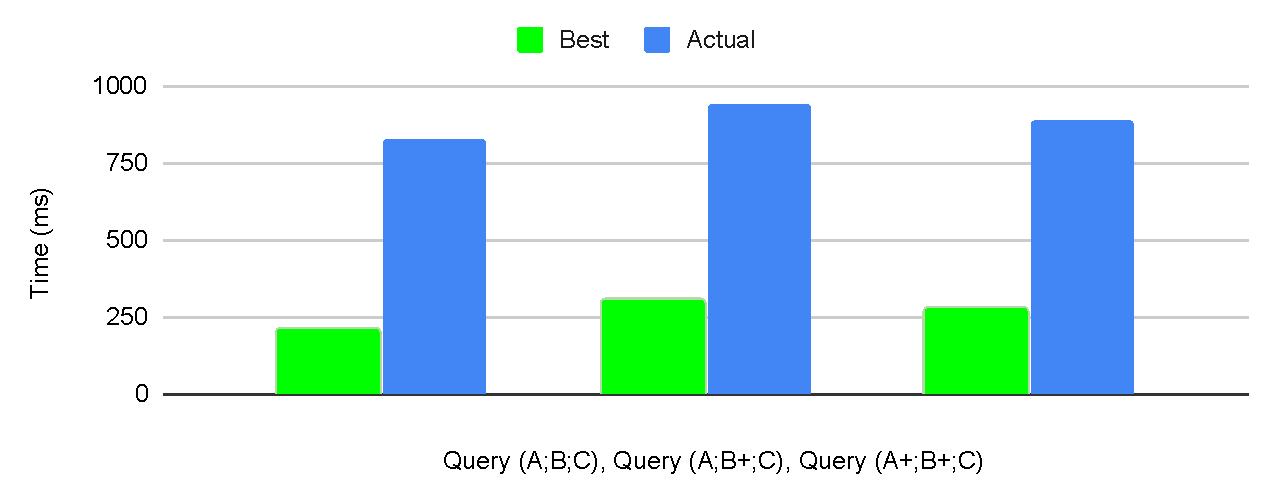
\includegraphics[scale=0.5]{experiment_5_chart_4}
  \caption{.}
  \label{fig:???}
\end{figure}

% 8 processors
\begin{figure}[H]
  \centering
  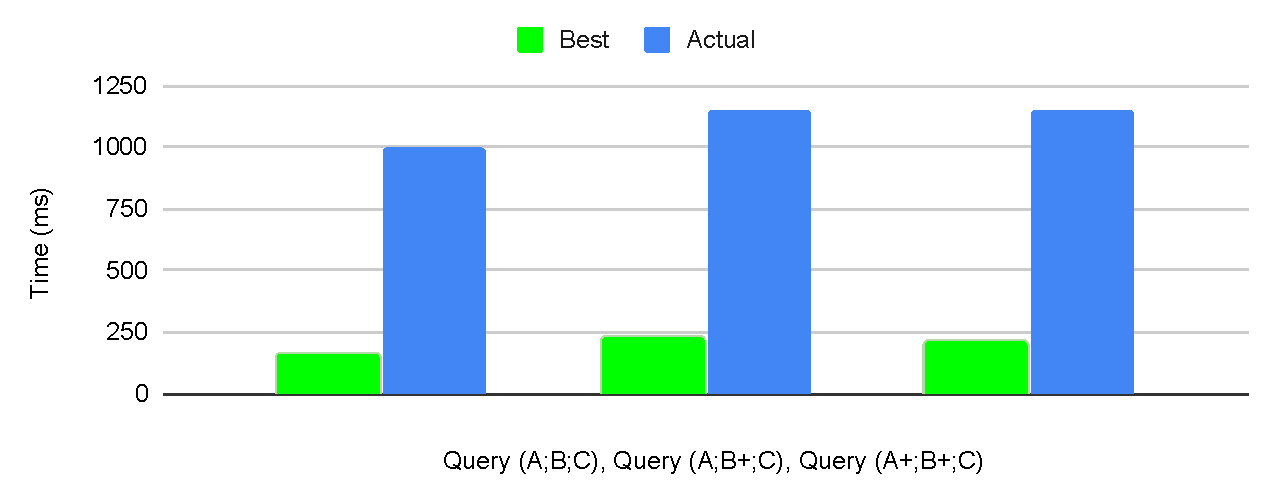
\includegraphics[scale=0.5]{experiment_5_chart_5}
  \caption{.}
  \label{fig:???}
\end{figure}

\textbf{Experimental results}.

\section{Chapter summary}
